\documentclass{article}
\usepackage[utf8]{inputenc}
\usepackage{esvect}
\usepackage{amsmath}
\usepackage[]{algorithm2e}
\usepackage{graphicx}
\usepackage{tabu}
\graphicspath{ {images/} }

\title{Predicting Box Office Performance for Movies}
\author{Sean Sodha (sss342), Anudeep Gavini(avg38), Omar Abdul-Rahim(oea5)}

\begin{document}

\maketitle

\section{Overview}

    We are using the “TMDB 5000 Movie Dataset” to analyze box office performance for movies. This dataset contains two files, “movies” and “credits.” The “movies” dataset contains information regarding movie title, genre, date, rating, budget, language, runtime, and our regression column of box office revenue, among other things. The “credits” dataset contains information regarding the entire cast and crew in listed order for each movie. We have joined these two datasets and below are some graphics that give an overview of the data. 
    
    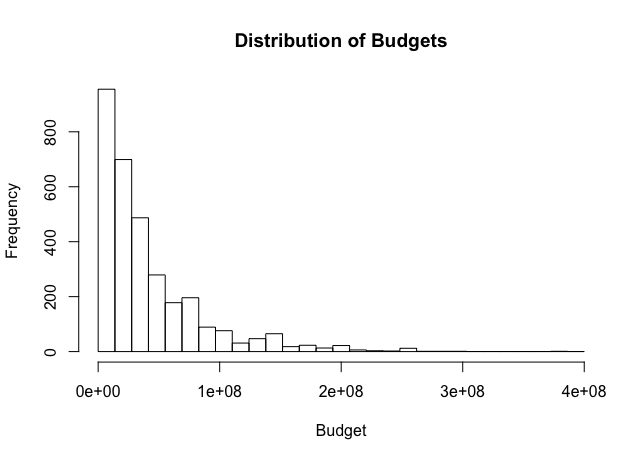
\includegraphics[scale=.25]{new_budget.png}
    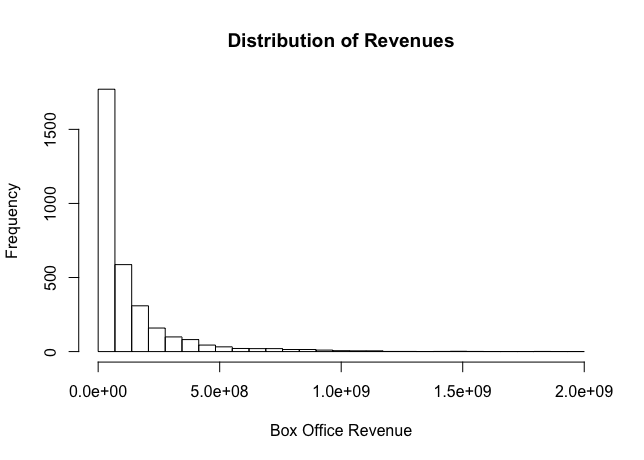
\includegraphics[scale=.25]{new_rating.png}
    
    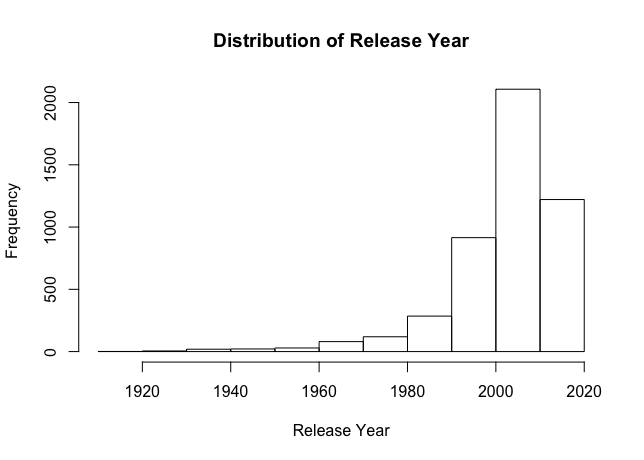
\includegraphics[scale=.25]{release.png}
    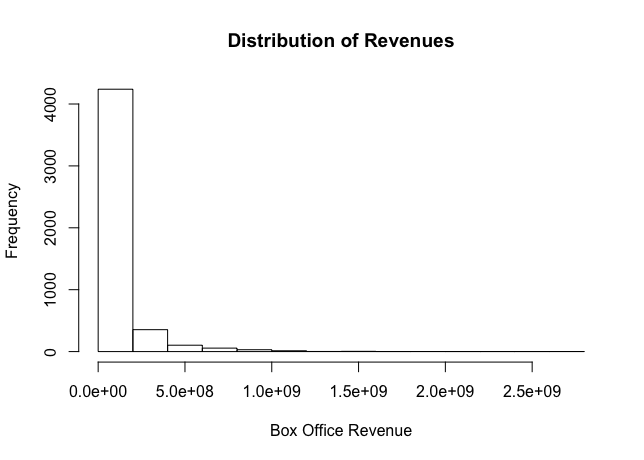
\includegraphics[scale=.25]{revenue.png}
    
    We have an excess of information as well as incomplete portions, so we must clean our data. As we progress through this report, we will explain what we did in order to clean the data and how we arrived to a clean dataset with usable information and features.

\section{Features}

    Originally, our dataset consisted of excess information such as the number of crew members, the language of the movie, etc. We cleaned up most of the data in Excel and we also noticed that many of the movies had a budget of \$0, a revenue of \$0, and some were missing both. We observed that those data points were mostly international movies and since we were focusing only on Hollywood movies, this would not affect our data so much. After eliminating movies with a budget and revenue of \$0, we were left with 3,200 movies which is still a substantial amount of data especially when we have amazing granularity in our data. Our Y matrix is the last column column.
    
    The following features will be used to predict the box office for movies: 

    \begin{table}[h!]

    \hspace*{-4.5cm}\begin{tabu} to \textwidth { |c|c|c|c|c|c|c|c| }
    \hline
     Movie Name & Director Awards & Genre & Director/Genre Relationship & Budget & Top 5 actors' Awards & Release Date & Revenue \\ 
     \hline
     $Movie_1$  & & & & & & & \\ 
     \hline
     $Movie_2$  & & & & & & & \\
     \hline
     . . .  & & & & & & & \\
     \hline
     $Movie_{3200}$ & & & & & & & \\
     \hline
    \end{tabu} 
    \end{table}
    
\section{Web Scraper}

    The only information that was given in our dataset for the actors was just their name. This does not help us to determine who would be the best actor to put in a movie. Therefore, we needed a way to quantify their performance in previous movies. Therefore, we implemented a web scraper in Python. Each actor has a unique ID on IMDB, so we first wrote a web scraper to retrieve the top 100,000 actor’s names as well as their unique ID. Now, each actor has a page of awards, so the web scraper searches that page for the total number of awards won, and then plots the data in a csv file. We have appended this data to the TMDB dataset that we obtained. 

\section{Over/Under Fitting}

Since we have around 3,200 data points, we are very unlikely going to underfit since we have so much data at our disposal. To avoid overfitting, we need to run multiple models and see if they are consistent or not. To first create our model, we will first train out model on about 2,500 (~80\%) movies in our data, and then we will test our model on the remaining 700 (~20\%) movie points. In addition, we will also run an n-fold cross-validation process to make sure that we test different types of data to see if we are consistent with our model or not. 

\section{Preliminary analysis}

The first thing we tried was running a linear regression of revenue against each of the numerical or categorical data in our set to check if there were any strongly positive or negative correlations between, say, the money a movie makes and the budget or runtime of the movie.  Graphs for these examples are below.

\hspace*{-3.5cm}
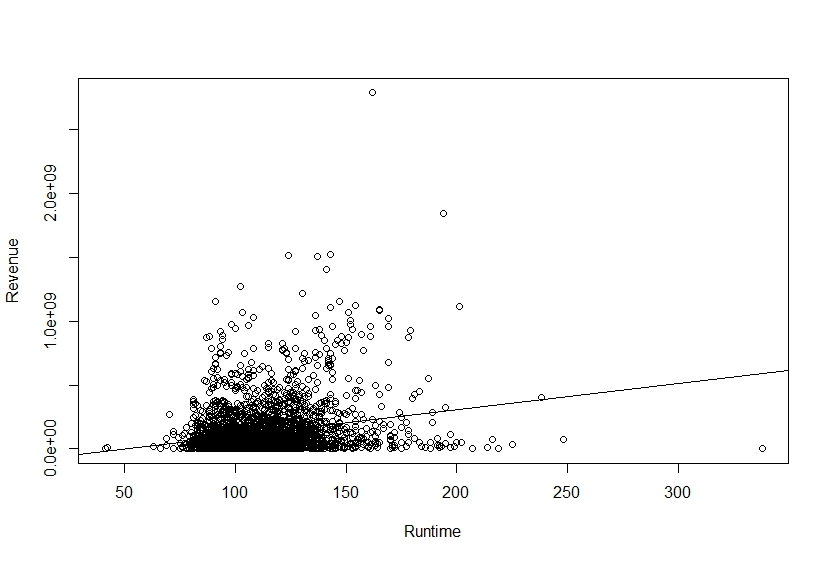
\includegraphics[scale = .4]{rvr.jpeg}
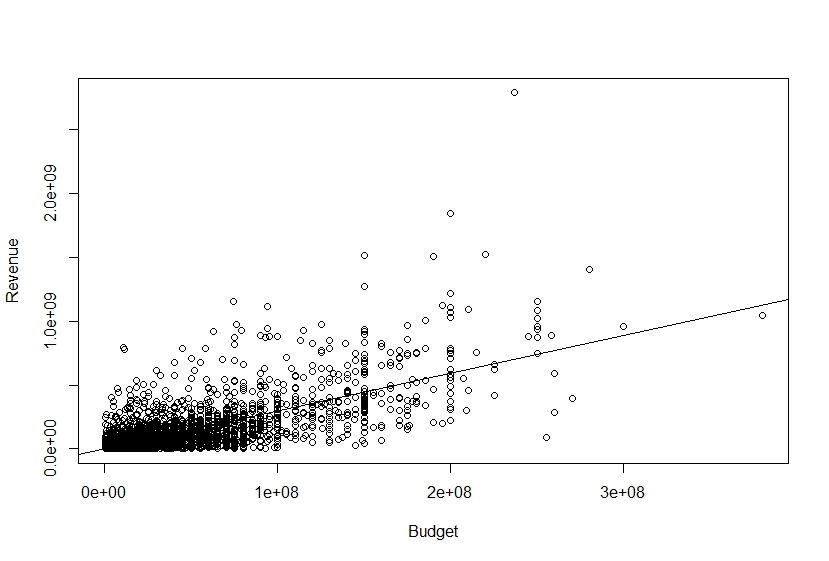
\includegraphics[scale = .4]{bvr.jpeg}

From just this, we can see that the amount of money put into a film has a larger impact than the runtime, as the revenue tends to increase with the budget, but the runtime graph looks more or less clustered with no real direction to the data.  Thus, we were able to remove some seemingly unrelated features from our data set, such as the runtime.  

We also wanted to run a similar regression analysis on the other columns as well, but these columns contained data unique to each movie - for example, the tagline, or the URL of the movie's webpage.  For these, we converted each observation into a boolean yes-or-no value that simply noted whether the value existed for each movie.  In this way we were able to construct a binomial regression analysis on each such feature, though we discovered that these features were also fairly uncorrelated with the revenue.

\section{Next Steps}

Our next steps are to find the correlation between directors and genres. We will rank every director in conjunction with every genre and see where they have performed the best. We will then assign a score to every rank for each actor where Rank 1 is where they perform best. In addition, we will then run some models on the data once we have fully quantified all of the data and perform validation tests on our model to test the accuracy. 

\end{document}
